\documentclass[journal,12pt,twocolumn]{IEEEtran}
%
\usepackage{setspace}
\usepackage{gensymb}
\usepackage{xcolor}
\usepackage{caption}
%\usepackage{subcaption}
%\doublespacing
\singlespacing
\usepackage{polynom}
%\usepackage{graphicx}
%\usepackage{amssymb}
%\usepackage{relsize}
\usepackage[cmex10]{amsmath}
\usepackage{mathtools}
%\usepackage{amsthm}
%\interdisplaylinepenalty=2500
%\savesymbol{iint}
%\usepackage{txfonts}
%\restoresymbol{TXF}{iint}
%\usepackage{wasysym}
\usepackage{hyperref}
\usepackage{amsthm}
\usepackage{mathrsfs}
\usepackage{txfonts}
\usepackage{stfloats}
\usepackage{cite}
\usepackage{cases}
\usepackage{subfig}
%\usepackage{xtab}
\usepackage{longtable}
\usepackage{multirow}
%\usepackage{algorithm}
%\usepackage{algpseudocode}
%\usepackage{enumerate}
\usepackage{enumitem}
\usepackage{mathtools}
%\usepackage{iithtlc}
%\usepackage[framemethod=tikz]{mdframed}
\usepackage{listings}


%\usepackage{stmaryrd}


%\usepackage{wasysym}
%\newcounter{MYtempeqncnt}
\DeclareMathOperator*{\Res}{Res}
%\renewcommand{\baselinestretch}{2}
\renewcommand\thesection{\arabic{section}}
\renewcommand\thesubsection{\thesection.\arabic{subsection}}
\renewcommand\thesubsubsection{\thesubsection.\arabic{subsubsection}}

\renewcommand\thesectiondis{\arabic{section}}
\renewcommand\thesubsectiondis{\thesectiondis.\arabic{subsection}}
\renewcommand\thesubsubsectiondis{\thesubsectiondis.\arabic{subsubsection}}

%\renewcommand{\labelenumi}{\textbf{\theenumi}}
%\renewcommand{\theenumi}{P.\arabic{enumi}}

% correct bad hyphenation here
\hyphenation{op-tical net-works semi-conduc-tor}

\lstset{
language=Python,
frame=single, 
breaklines=true,
columns=fullflexible
}



\begin{document}
%

\theoremstyle{definition}
\newtheorem{theorem}{Theorem}[section]
\newtheorem{problem}{Problem}
\newtheorem{proposition}{Proposition}[section]
\newtheorem{lemma}{Lemma}[section]
\newtheorem{corollary}[theorem]{Corollary}
\newtheorem{example}{Example}[section]
\newtheorem{definition}{Definition}[section]
%\newtheorem{algorithm}{Algorithm}[section]
%\newtheorem{cor}{Corollary}
\newcommand{\BEQA}{\begin{eqnarray}}
\newcommand{\EEQA}{\end{eqnarray}}
\newcommand{\define}{\stackrel{\triangle}{=}}
\bibliographystyle{IEEEtran}
%\bibliographystyle{ieeetr}
\providecommand{\nCr}[2]{\,^{#1}C_{#2}} % nCr
\providecommand{\nPr}[2]{\,^{#1}P_{#2}} % nPr
\providecommand{\mbf}{\mathbf}
\providecommand{\pr}[1]{\ensuremath{\Pr\left(#1\right)}}
\providecommand{\qfunc}[1]{\ensuremath{Q\left(#1\right)}}
\providecommand{\sbrak}[1]{\ensuremath{{}\left[#1\right]}}
\providecommand{\lsbrak}[1]{\ensuremath{{}\left[#1\right.}}
\providecommand{\rsbrak}[1]{\ensuremath{{}\left.#1\right]}}
\providecommand{\brak}[1]{\ensuremath{\left(#1\right)}}
\providecommand{\lbrak}[1]{\ensuremath{\left(#1\right.}}
\providecommand{\rbrak}[1]{\ensuremath{\left.#1\right)}}
\providecommand{\cbrak}[1]{\ensuremath{\left\{#1\right\}}}
\providecommand{\lcbrak}[1]{\ensuremath{\left\{#1\right.}}
\providecommand{\rcbrak}[1]{\ensuremath{\left.#1\right\}}}
\theoremstyle{remark}
\newcommand\Mydiv[2]{%
$\strut#1$\kern.25em\smash{\raise.3ex\hbox{$\big)$}}$\mkern-8mu
        \overline{\enspace\strut#2}$}
\newtheorem{rem}{Remark}
\newcommand{\sgn}{\mathop{\mathrm{sgn}}}
\providecommand{\abs}[1]{\left\vert#1\right\vert}
\providecommand{\res}[1]{\Res\displaylimits_{#1}} 
\providecommand{\norm}[1]{\lVert#1\rVert}
\providecommand{\mtx}[1]{\mathbf{#1}}
\providecommand{\mean}[1]{E\left[ #1 \right]}
\providecommand{\fourier}{\overset{\mathcal{F}}{ \rightleftharpoons}}
\providecommand{\ztrans}{\overset{\mathcal{Z}}{ \rightleftharpoons}}
\newcommand{\myvec}[1]{\ensuremath{\begin{pmatrix}#1\end{pmatrix}}}
\newcommand{\mydet}[1]{\ensuremath{\begin{vmatrix}#1\end{vmatrix}}}
%\providecommand{\hilbert}{\overset{\mathcal{H}}{ \rightleftharpoons}}
\providecommand{\system}{\overset{\mathcal{H}}{ \longleftrightarrow}}
	%\newcommand{\solution}[2]{\textbf{Solution:}{#1}}
\newcommand{\solution}{\noindent \textbf{Solution: }}
\providecommand{\dec}[2]{\ensuremath{\overset{#1}{\underset{#2}{\gtrless}}}}
\numberwithin{equation}{section}
%\numberwithin{equation}{subsection}
%\numberwithin{problem}{subsection}
%\numberwithin{definition}{subsection}
\makeatletter
\@addtoreset{figure}{problem}
\makeatother
\let\StandardTheFigure\thefigure
%\renewcommand{\thefigure}{\theproblem.\arabic{figure}}
\renewcommand{\thefigure}{\theproblem}
%\numberwithin{figure}{subsection}
\def\putbox#1#2#3{\makebox[0in][l]{\makebox[#1][l]{}\raisebox{\baselineskip}[0in][0in]{\raisebox{#2}[0in][0in]{#3}}}}
     \def\rightbox#1{\makebox[0in][r]{#1}}
     \def\centbox#1{\makebox[0in]{#1}}
     \def\topbox#1{\raisebox{-\baselineskip}[0in][0in]{#1}}
     \def\midbox#1{\raisebox{-0.5\baselineskip}[0in][0in]{#1}}
\vspace{3cm}
\vspace{3cm}
\title{Digital Signal Processing}
\author{sumeeth kumar} 
% make the title area
\maketitle
%\newpage
\tableofcontents
\renewcommand{\thefigure}{\theenumi}
\renewcommand{\thetable}{\theenumi}
%\renewcommand{\theequation}{\thesection}
\bigskip
\begin{abstract}
This manual provides a simple introduction to digital signal processing.
\end{abstract}
\noindent \section{Software Installation}
\noindent Run the following commands (commands may change depending on Linux distro)
\begin{lstlisting}
$ sudo apt update && sudo apt upgrade
$ sudo apt install libffi-dev libsndfile1 python3-scipy python3-numpy python3-matplotlib 
$ pip3 install cffi pysoundfile 
\end{lstlisting}
\section{Digital Filter}
\begin{enumerate}[label=\thesection.\arabic*
,ref=\thesection.\theenumi]
\item
\label{prob:input}
Download the sound file using
\begin{lstlisting}
$https://github.com/sumeethkumar12/signal-processing/blob/main/Sound_With_ReducedNoise.wav
\end{lstlisting}
\item
\label{prob:spectrogram}
You will find a spectrogram at \href{https://academo.org/demos/spectrum-analyzer}{\url{https://academo.org/demos/spectrum-analyzer}}. Upload the sound file that you downloaded in Problem \ref{prob:input} in the spectrogram and play. Observe the spectrogram. What do you find?
\solution There are a lot of yellow lines between 440 Hz to 5.1 KHz.  These represent the synthesizer key tones. Also, the key strokes
are audible along with background noise.
\item
\label{prob:output}
Write the python code for removal of out of band noise and execute the code.\\
\solution
Download the source code using
\begin{lstlisting}
$ https://github.com/sumeethkumar12/signal-processing/blob/main/codes/cancel_noise.py
\end{lstlisting}
and execute it using
\begin{lstlisting}
$ python3 cancel_noise.py
\end{lstlisting}
\item
The output of the python script in Problem \ref{prob:output} is the audio file \texttt{Sound\_With\_ReducedNoise.wav}. Play the file in the spectrogram in Problem \ref{prob:spectrogram}. What do you observe?\\
\solution The key strokes as well as background noise is subdued in the audio. Also, the signal is blank for frequencies above 5.1 kHz.
\end{enumerate}
\section{Difference Equation}
\begin{enumerate}[label=\thesection.\arabic*,ref=\thesection.\theenumi]
\item Let
\begin{equation}
x(n) = \cbrak{\underset{\uparrow}{1},2,3,4,2,1}
\end{equation}
Sketch $x(n)$.
\item Let
\begin{multline}
\label{eq:iir_filter}
y(n) + \frac{1}{2}y(n-1) = x(n) + x(n-2), 
\\
y(n) = 0, n < 0
\end{multline}
Sketch $y(n)$.\\
\solution The following code yields Fig. \eqref{fig:xnyn}.
\begin{lstlisting}
$ https://github.com/sumeethkumar12/signal-processing/blob/main/codes/xnyn.py
\end{lstlisting}
and execute it using
\begin{lstlisting}
$ python3 xnyn.py
\end{lstlisting}
\begin{figure}[!ht]
	\centering
	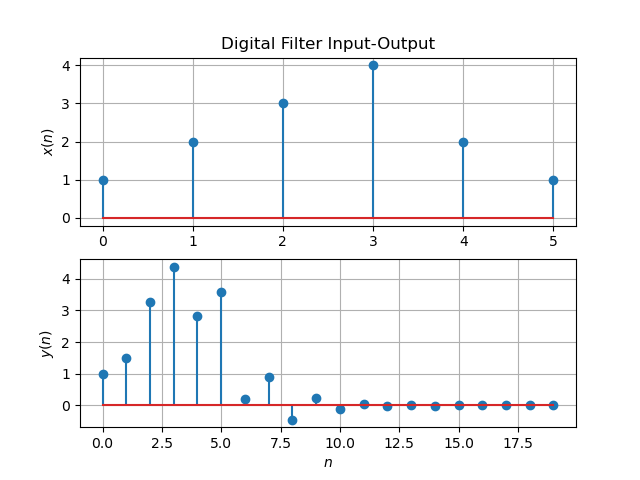
\includegraphics[width=\columnwidth]{xnyn.png}
	\caption{Plot of $x(n)$ and $y(n)$}
	\label{fig:xnyn}
\end{figure}
\item Repeat the above exercise using a C code.
\begin{lstlisting}
$ https://github.com/sumeethkumar12/signal-processing/blob/main/codes/xnyn.c
\end{lstlisting}

\end{enumerate}
\section{$Z$-transform}
\begin{enumerate}[label=\thesection.\arabic*]
\item The $Z$-transform of $x(n)$ is defined as 
%
\begin{equation}

X(z)={\mathcal {Z}}\{x(n)\}=\sum _{n=-\infty }^{\infty }x(n)z^{-n}
\end{equation}
%
Show that
\begin{equation}
{\mathcal {Z}}\{x(n-1)\} = z^{-1}X(z)
\end{equation}
and find
\begin{equation}
	{\mathcal {Z}}\{x(n-k)\} 
\end{equation}
\solution Given that,
  \begin{align}
     X\brak{z} &= \mathcal{Z}\cbrak{x\brak{n}}\\
               &= \sum_{n = -\infty}^{\infty}x\brak{n}z^{-n}
  \end{align}
  So,
   \begin{align}
     \mathcal{Z}\cbrak{x\brak{n-1}} &= \sum_{n=-\infty}^{\infty}x\brak{n-1}z^{-n}
   \end{align}
   Take $k = n-1$,
   \begin{align}
           &= \sum_{k=-\infty}^{\infty}x\brak{k}z^{-\brak{k+1}}\\
           &= z^{-1}\sum_{k=-\infty}^{\infty}x\brak{k}z^{-k}\\
           &= z^{-1}\sum_{n=-\infty}^{\infty}x\brak{n}z^{-n}\\
           &= z^{-1}X\brak{z}    
   \end{align}
   resulting in  and similarly following the above steps you will get,
     \begin{align}
          \mathcal{Z}\cbrak{x\brak{n-k}} &= z^{-k}X\brak{n}\label{shift_k_Z_transform}
     \end{align} 
\item
   Now we will find $Z$ transform of the signal 
    \begin{align}
      \mathcal{Z}\cbrak{x\brak{n}} &= \sum_{n=0}^{5}x\brak{n}z^{-n}\\
                                   &= 1z^{0} + 2z^{-1} + 3z^{-2}+4z^{-3} + 2z^{-4} +1z^{-5}\\
                                   &= 1 + 2z^{-1} + 3z^{-2} + 4z^{-3} + 2z^{-4} + z^{-5} 
    \end{align}
   \item Find
   %
   \begin{equation}
   H(z) = \frac{Y(z)}{X(z)}
   \end{equation}
   %
   from  $\eqref{eq:iir_filter}$ assuming that the $Z$-transform is a linear operation.
   \\
   \solution 
   \begin{align}
   Y(z) + \frac{1}{2}z^{-1}Y(z) &= X(z)+z^{-2}X(z)
   \\
   \implies \frac{Y(z)}{X(z)} &= \frac{1 + z^{-2}}{1 + \frac{1}{2}z^{-1}}
   \label{eq:freq_resp}
   \end{align}
   %
    \solution 
     Now we will rewrite ,
      \begin{align}
          y(n) + \frac{1}{2}y(n-1) = x(n) + x(n-2)
      \end{align}
     Now since $Z$-transform is a linear operator we can write that,
      \begin{align}
          Y\brak{n} + \frac{1}{2}Y\brak{n-1} &= X\brak{n} + X\brak{n-2}
      \end{align}

      \begin{align}
          Y\brak{n} + \frac{z^{-1}}{2}Y\brak{n} &= X\brak{n} + z^{-2}X\brak{n}\\
       \implies \frac{Y\brak{n}}{X\brak{n}} &= \frac{1 + z^{-2}}{1 + \frac{z^{-1}}{2}} 
      \end{align}       
      \item Find the Z transform of 
      \begin{equation}
      \label{delta}
      \delta(n)
      =
      \begin{cases}
      1 & n = 0
      \\
      0 & \text{otherwise}
      \end{cases}
      \end{equation}
      and show that the $Z$-transform of
      \begin{equation}
      \label{eq:unit_step}
      u(n)
      =
      \begin{cases}
      1 & n \ge 0
      \\
      0 & \text{otherwise}
      \end{cases}
      \end{equation}
      is
      \begin{equation}
      U(z) = \frac{1}{1-z^{-1}}, \quad \abs{z} > 1
      \end{equation}
      \solution 
      The $Z$-transform of $\delta{n}$ is,
      \begin{align}
          \mathcal{Z}\cbrak{\delta{n}} &= \sum_{n=-\infty}^{\infty}\delta\brak{n}z^{-n}\\
                                       &= \delta\brak{0}z^{0} + 0\,\, \brak{\text{Using \eqref{delta}}}\\
                                       &= 1
      \end{align}
       and the $Z$-transform of unit-step function $u\brak{n}$ is,
      \begin{align}
          U\brak{n} &= \sum_{n=-\infty}^{\infty}u\brak{n}z^{-n}\\
                    &= 0 + \sum_{n = 0}^{\infty}1.z^{-n}\\
                    &= 1 + z^{-1} + z^{-2} + .\,.\,.
      \end{align}
       Above is a infinite geometric series with $z^{-1}$ as common ratio , so we can write it as 
      \begin{align}
          U\brak{n} &= \frac{1}{1-z^{-1}} \because \abs{z} > 1
      \end{align} 
    \item Show that 
      \begin{equation}
        \label{eq:anun}
        a^nu(n) \ztrans \frac{1}{1-az^{-1}} \quad \abs{z} > \abs{a}
      \end{equation}
    \solution
     The $Z$- transform will be 
      \begin{align}
              \mathcal{Z}\cbrak{a^nu\brak{n}} &= \sum_{n = 0}^{\infty}a^{n}z^{-n}\\
                                              &= 1 + \frac{a}{z} + \brak{\frac{a}{z}}^2 + .\,.\,.\,.
      \end{align}
     Above is a infinite geometric series with first term $1$ and common ratio as $\frac{a}{z}$ and it can 
       be written as,
      \begin{align}
              \mathcal{Z}\cbrak{a^nu\brak{n}} &= \frac{1}{1 - \frac{a}{z}} \because \abs{a} < \abs{z} 
      \end{align}
     Therefore,
      \begin{equation}
          a^nu(n) \ztrans \frac{1}{1-az^{-1}} \quad \abs{z} > \abs{a}
      \end{equation}

\item
1et
\begin{equation}
H\brak{e^{\j \omega}} = H\brak{z = e^{\j \omega}}.
\end{equation}
Plot $\abs{H\brak{e^{\j \omega}}}$.  Comment.  $H(e^{\j \omega})$ is
known as the {\em Discret Time Fourier Transform} (DTFT) of $x(n)$.
\solution The following code plots Fig. .
\begin{lstlisting}
$ https://github.com/sumeethkumar12/signal-processing/blob/main/codes/dtft.py
\end{lstlisting}
The figure can be generated using
\begin{lstlisting}
$ python3 dtft.py
\end{lstlisting}
We observe that $\left|H\brak{e^{j\omega}}\right|$ is periodic with fundamental period 2$\pi$.
\begin{figure}[!ht]
	\centering
	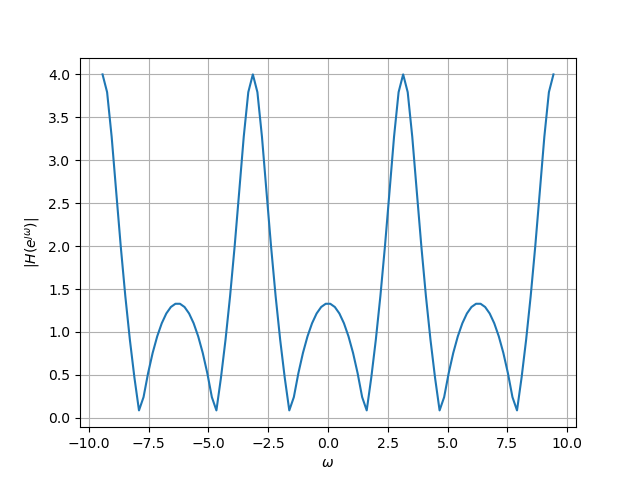
\includegraphics[width=\columnwidth]{dtft.png}
	\caption{Plot of $\left|H\brak{e^{j\omega}}\right|$ against $\omega$}
	\label{fig:H-w}
\end{figure}
Now using  we will find $\abs{H\brak{e^{j \omega}}}$,
     \begin{align}
      H\brak{e^{j \omega}} &= \frac{1+e^{-2j\omega}}{1 + \frac{e^{-j\omega}}{2}}\\
        \implies \abs{H\brak{e^{j \omega}}} &= \frac{\abs{1+e^{-2j\omega}}}{\abs{1 + \frac{e^{-j\omega}}{2}}}\\
                            &= \frac{\abs{1+e^{2j\omega}}}{\abs{e^{2j\omega} + \frac{e^{j\omega}}{2}}}\\
                            &= \frac{\abs{1+\cos2\omega + j\sin2\omega}}{\abs{e^{j\omega}+ \frac{1}{2}}}\\
                            &= \frac{\abs{4\cos^2\brak{\omega} + 4j\sin\brak{\omega}\cos\brak{\omega}}}{\abs{2e^{j\omega} + 1}}\\
                            &= \frac{\abs{4\cos\brak{\omega}}\abs{\cos\brak{\omega} + j\sin\brak{\omega}}}{\abs{2\cos\brak{\omega} + 1 + 2j\sin\brak{\omega}}}\\
        \therefore \abs{H\brak{e^{j \omega}}} &= \frac{\abs{4\cos\brak{\omega}}}{\sqrt{5 +4\cos\brak{\omega}}}
     \end{align}
      Using the above expression we can say that graph is symmetric about origin and has a period of $2\pi$.
  \item Express $h(n)$ in terms of $H\brak{e^{j \omega}}$.\\

	\solution 
	\begin{align}
		&\int_{-\pi}^{\pi} H(e^{\j\omega}) e^{\j\omega n} \der{\omega} \\
		&= \int_{-\pi}^{\pi} \sum_{k=-\infty}^\infty h(k)  e^{-\j\omega k} e^{\j\omega n} \der{\omega} \\
		&= \sum_{k=-\infty}^\infty h(k) \int_{-\pi}^{\pi} e^{\j\omega(n-k)} \der{\omega}
	\end{align}
	
	Now,
	\begin{align}
		 \int_{-\pi}^{\pi} e^{\j\omega(n-k)} \der{\omega} 
		 &= \begin{cases}
		 	\int_{-\pi}^\pi \der{\omega} & n-k = 0 \\
		 	\left.\frac{\exp\brak{\j\omega(n-k)}}{\j(n-k)}\right|_{-\pi}^\pi & n-k \ne 0
		 \end{cases} \\		 
		 &= \begin{cases}
		 	2\pi & n-k = 0 \\
		 	0 & n-k \ne 0
		 \end{cases} \\
		 &= 2\pi \delta(n-k)
	\end{align}
	
	Thus,
	\begin{align}
		\int_{-\pi}^{\pi} H(e^{\j\omega}) e^{\j\omega n} \der{\omega} &= 2\pi\sum_{k=-\infty}^\infty h(k) \delta(n-k) \\
		&= 2\pi h(n) * \delta(n) \\
		&= 2\pi h(n)
	\end{align}
	
	Therefore, $h(n)$ is given by the inverse DTFT (IDTFT) of $H\brak{e^{\j\omega}}$
	\begin{align}
		h(n) &= \frac{1}{2\pi} \int_{-\pi}^{\pi} H(e^{\j\omega}) e^{\j\omega n} \der{\omega} 
	\end{align}
\end{enumerate}
\section{Impulse Response}
  \begin{enumerate}[label=\thesection.\arabic*]
    \item Using long division, 
find
		\begin{align}
			h(n), \quad n < 5
		\end{align}
		for H(z) in 
		.\\
    \solution  we can write
	  \begin{align}
		H\brak{z} &= \frac{1 + z^{-2}}{1 + \frac{z^{-1}}{2}}
	  \end{align}
    $$
\begin{array}{llllll}
& 2z^{-1} & -4 \\\cline{2-5}
1 + z^{-1}/2 | & 1& +z^{-2}  \\
& 2z^{-1} & +z^{-2}  \\\cline{2-5}
& & 1 & -2z^{-1} \\
& & -4 & -2z^{-1} & \\\cline{3-5}
& & & 5 \\
\end{array}
$$
So we can replace as, 
   \begin{align}
     \frac{1+z^{-2}}{1 + \frac{z^{-1}}{2}} &= 2z^{-1} - 4 + \frac{5}{1 + z^{-1}/2}\label{eq:longdiv}
   \end{align}
   Now we can expand the second term of above expression as an infinite geometric series,
   \begin{align}
     \frac{5}{1+z^{-1}/2} &= 5\brak{1 + \brak{\frac{-1}{2z}} + \brak{\frac{-1}{2z}}^2 + .\,.\,.} 
    \end{align}
     where we assume $\abs{\frac{1}{2z}} < 1$.\\
ROC is $|z|>\frac{1}{2}$.\\
    So  will become,
    \begin{align}
      &= 2z^{-1} - 4 + 5 + \frac{-5}{2}z^{-1} + \frac{5}{4}z^{-2} + \frac{-5}{8}z^{-3} + \frac{5}{16}z^{-4} + \,.\,.\\
      &= 1z^{0} + \frac{-1}{2}z^{-1} +\frac{5}{4}z^{-2} + \frac{-5}{8}z^{-3} +\frac{5}{16}z^{-4} + \,.\,.  \label{eq:longdiv_exp}
    \end{align}
   Now to get $h(n)$ for $n <5$ we will compare with the below equation,
    \begin{align}
      H\brak{z} &= \sum_{n = -\infty}^{n = \infty}h(n)z^{-n}
    \end{align}
    $h(n)$ will be the coefficient of $z^{-n}$.\\
     Using this, we can write,
     \begin{align}
      h(0) &= 1\\
      h(1) &= \frac{-1}{2}\\
      h(2) &= \frac{5}{4}\\
      h(3) &= \frac{-5}{8}\\
      h(4) &= \frac{5}{16}
     \end{align}
     And for $n<0\,\, h(n) = 0$.\\
     For $n>5$, we can get h\brak{n} from the geometric series,
      \begin{align}
        h\brak{n} &= 5\brak{\frac{-1}{2}}^n
      \end{align}
    \item \label{prob:impulse_resp}
      Find an expression for $h(n)$ using $H(z)$, given that 
     
      \begin{equation}
        
        h(n) \ztrans H(z)
      \end{equation}
      and there is a one to one relationship between $h(n)$ and $H(z)$. $h(n)$ is known as the {\em impulse response} of the system defined .\\ 
    \solution The $H\brak{z}$ can be written as,
      \begin{align}
         H\brak{z} &= \frac{1}{1 + \frac{z^{-1}}{2}} + \frac{z^{-2}}{1+\frac{z^{-1}}{2}}
      \end{align}
       we can write it as,
      \begin{align}
        h\brak{n} &= \brak{\frac{-1}{2}}^{n} u\brak{n} + \brak{\frac{-1}{2}}^{n-2} u\brak{n-2}\label{eq:hn}
      \end{align}
    \item Sketch $h(n)$. Is it bounded? Justify Theoritically.\\
    \solution  Download the code for the plot  from the below link,
     \begin{lstlisting}
wget https://github.com/sumeethkumar12Signal_Processing/blob/master/Sound%201/Codes/hn.py
     \end{lstlisting}
     \begin{figure}[ht!]
      \centering
      \includegraphics[width = \columnwidth]{hn.png}
      \caption{$h\brak{n}$ as inverse of $H\brak{n}$}     
      \label{hn}
     \end{figure}
     From the plot it seems like $h(n)$ is bounded and becomes smaller in magnitude as $n$ increases.\\
    Using , we can get theoritical expression as, 
     \begin{align}
       h\brak{n} &= \begin{cases}
                        0 &, n < 0\\
                        \brak{\frac{-1}{2}}^n &, 0\leq n<2\\
                        5\brak{\frac{-1}{2}}^n &, n \geq 2
                     \end{cases}\label{eq:hn_theo}
     \end{align}
    A sequence $\cbrak{x_n}$ is said to be bounded if and only if there exist a positive real number $M$ such that,
         \begin{align}
           \abs{x_n} \leq M , \forall n \in \mathcal{N}\label{def:bounded}
         \end{align}      
    So to say $h\brak{n}$ is bounded we should able to find the $M$ which satisfies .\\
    For $n < 0$, 
       \begin{align}
    \abs{h\brak{n}} \leq 0 
       \end{align}
    For $0 \leq n <2$,
       \begin{align}
        \abs{h\brak{n}} &= \abs{\frac{-1}{2}}^{n}\\
                        &= \brak{\frac{1}{2}}^{n} \leq 1
       \end{align}
    And for $n \geq 2$,
       \begin{align}
        \abs{h\brak{n}} &= \abs{5\brak{\frac{-1}{2}}}^{n}\\
                        &= \brak{\frac{5}{2}}^{n} \leq \frac{5}{4}
       \end{align}
    From above three cases, we can get $M$ as,
      \begin{align}
        M &= max\cbrak{0,1,\frac{5}{4}} \\
          &= \frac{5}{4}
      \end{align}
    Therefore, $h\brak{n}$ is bounded  with $M = \frac{5}{4}$ i.e.,
    \begin{align} 
      \abs{h(n)} \leq \frac{5}{4}  \forall n \in \mathcal{N}
    \end{align}    
     \item Convergent? Justify using the ratio test.\\
     \solution We can say a given real sequence $\cbrak{x_n}$ is convergent if 
       \begin{align}
         \lim_{n \rightarrow \infty}\abs{\frac{x_{n+1}}{x_n}} < 1
       \end{align}
        This is known as Ratio test.\\
      In this case the limit will become,
       \begin{align}
         \lim_{n \rightarrow \infty}\abs{\frac{h\brak{n+1}}{h\brak{n}}} &= \lim_{n \rightarrow \infty}\abs{\frac{5\brak{\frac{-1}{2}}^{n+1}}{5\brak{\frac{-1}{2}}^{n}}} \\
          &= \lim_{n \rightarrow \infty}\abs{\frac{-1}{2}}\\
          &= \frac{1}{2}
       \end{align}
      As $\frac{1}{2} < 1$, from root test we can say that $h\brak{n}$ is convergent.
       \item The system with $h(n)$ is defined to be stable if
     \begin{equation}
      \sum_{n=-\infty}^{\infty}h(n) < \infty
     \end{equation}
        Is the system defined  stable for the impulse response ?\\
    \solution ,
      \begin{align}
        \sum_{n=-\infty}^{\infty}h\brak{n} &= \sum_{n=-\infty}^{\infty}\brak{\brak{\frac{-1}{2}}^{n} u\brak{n} + \brak{\frac{-1}{2}}^{n-2} u\brak{n-2}}\\
                                           &= 2\brak{\frac{1}{1+\frac{1}{2}}}\\
                                           &= \frac{4}{3}
      \end{align}
       $\therefore$ the system is stable.  
    \item Verify the above result using a python code.\\
    \solution Download the python code from the below link 
    \begin{lstlisting}
  wget https://github.com/sumeethkumar12/Signal_Processing/blob/master/Sound%201/Codes/hnstable.py
    \end{lstlisting}
  Then run the following command,
    \begin{lstlisting}
  python3 hn_stable.py
    \end{lstlisting} 
    \item Compute and sketch $h(n)$ using 
     \begin{equation}
      h(n) + \frac{1}{2}h(n-1) = \delta(n) + \delta(n-2), 
     \end{equation}
        This is the definition of $h(n)$.\\
    \solution Download the code for the plot \ref{hndef} from the below link,
     \begin{lstlisting}
wget https://github.com/sumeethkumar12/Signal_Processing Codes/hndef.py
     \end{lstlisting}
     Note that this is same as $\ref{hn}$.\\
     \begin{figure}[ht!]
      \centering
      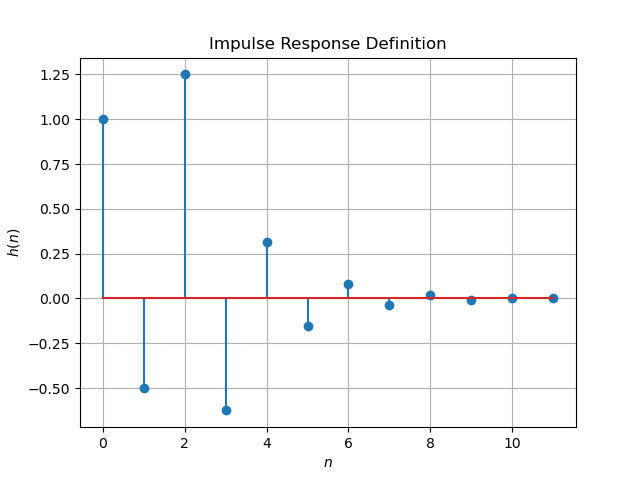
\includegraphics[width = \columnwidth]{hndef.png}
      \caption{From the definition of $h(n)$}
     \end{figure}
    For $n <0$, $h\brak{n} = 0$ and,
     \begin{align} 
       h\brak{0} &= \delta\brak{0}\\
                 &= 1
     \end{align}
    For $n =1$,
     \begin{align} 
       h\brak{1} + \frac{1}{2}h\brak{0} &= \delta\brak{1} + \delta\brak{-1}\\
      \implies  h\brak{1}&= -\frac{1}{2}h\brak{0}\\
                         &= -\frac{1}{2}
     \end{align}
    $n=2$,
      \begin{align}
        h\brak{2} + \frac{1}{2}h\brak{1} &= 0 + \delta\brak{0}\\
              h\brak{2} &= 1 + \frac{1}{4}\\
                        &= \frac{5}{4}
      \end{align}
    And for $n>2$ RHS will be $0$ so,
      \begin{align}
        h\brak{n} &= -\frac{1}{2}h\brak{n-1}
      \end{align}
    Overall 
      \begin{align}
         h\brak{n} &= \begin{cases}
                          0  &, n <0 \\
                          1  &, n = 0 \\
                        -\frac{1}{2} &, n=1 \\
                        \frac{5}{4} &, n =2\\
                        -\frac{1}{2}h\brak{n-1} &, n >2
         \end{cases}
         \end{align}
        \item Compute 
     %
     \begin{equation}
     \label{eq:convolution}
     y(n) = x(n)*h(n) = \sum_{k=-\infty}^{\infty}x(k)h(n-k)
     \end{equation}
     %
     Comment. The operation  is known as
     {\em convolution}.\\
     %
     \solution Download the code for plot from the below link
      \begin{lstlisting}
wget https://github.com/sumeethkumar12Signal_Processing/blob/master/Sound%201/Codes/ynconv.py
      \end{lstlisting}
      Note that the plot is same that as in .
      \begin{figure}[ht!]
        \centering
        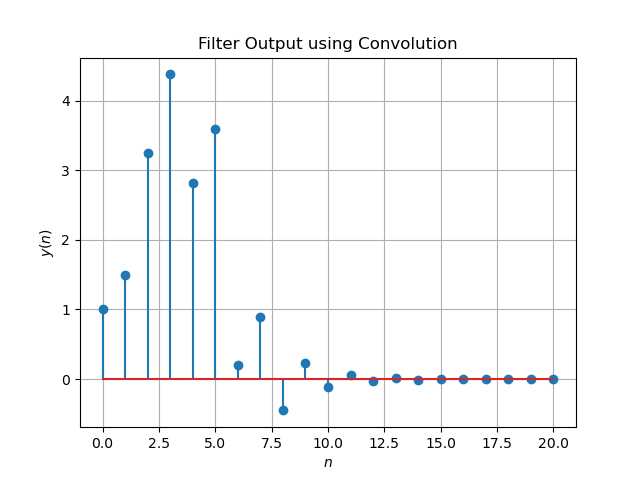
\includegraphics[width = \columnwidth]{ynconv.png}
        \caption{$y(n)$ using the convolution definition}
        \label{ynconv}
      \end{figure}
    \item Express the above convolution using a Toeplitz matrix.\\
    \solution Download the python code from the below link for the plot,
     \begin{lstlisting}
wget https://github.com/sumeethkumar12Signal_Processing/blob/master/Sound%201/Codes/ynconv_toeplitz.py
     \end{lstlisting}
    Then run the following command,
     \begin{lstlisting}
python3 ynconv_toeplitz.py
     \end{lstlisting}
    we express $y\brak{n}$ as
     \begin{align}
       y\brak{n} &= \sum_{k = -\infty}^{\infty}x\brak{k}h\brak{n-k}
     \end{align}
    To understand how we can use a Toeplitz matrix, we will see what we are doing in 
     \begin{align}
      y\brak{0} &= x\brak{0}h\brak{0}\\
      y\brak{1} &= x\brak{0}h\brak{1} + x\brak{1}h\brak{0}\\
      y\brak{2} &= x\brak{0}h\brak{2} + x\brak{1}h\brak{1} + x\brak{2}h\brak{0}\\
      . \nonumber&\\ 
      .& \nonumber
     \end{align}
    The same thing can be written as,
     \begin{align}
       y\brak{0} &= \myvec{h\brak{0} & 0 & 0 &.\,&.\,&.0}\myvec{x\brak{0}\\x\brak{1}\\x\brak{2}\\ . \\.\\x\brak{5}}\\
       y\brak{1} &= \myvec{h\brak{1} & h\brak{0} & 0 & 0 &.\,&.\,&.0}\myvec{x\brak{0}\\x\brak{1}\\x\brak{2}\\ . \\.\\x\brak{5}}\\
       y\brak{2} &= \myvec{h\brak{2} & h\brak{1} & h\brak{0} & 0& .\,&.0}\myvec{x\brak{0}\\x\brak{1}\\x\brak{2}\\ . \\.\\x\brak{5}}\\
       . & \nonumber \\
       .& \nonumber
     \end{align}
    Using Toeplitz matrix of $h\brak{n}$ we can simplify it as,
     \begin{align}
       y\brak{n} &= \myvec{h\brak{0} & 0 & 0 &.\,&.\,&.\,0 \\
                           h\brak{1} & h\brak{0} & 0 & .\,&.\,&.\,0 \\
                           h\brak{2} & h\brak{1} & h\brak{0} & .\,&.\,&.\,0 \\
                            &&..\\&&..\\ 0 & 0 &  0 &.\,&.\,&.\, h\brak{m-1}}\myvec{x\brak{0}\\x\brak{1}\\x\brak{2}\\ . \\.\\x\brak{5}}
     \end{align}
     Now  we will take n 
      \begin{align}
          x\brak{n} &= \myvec{1\\2\\3\\4\\2\\1}
      \end{align}
      And ,
      \begin{align} 
        h\brak{n} &= \myvec{1 \\ -0.5 \\ 1.25 \\. \\ . }
      \end{align}
     Now ,
      \begin{align}
        y\brak{n} &= x\brak{n}*h\brak{n}\\
                  &= \myvec{1 & 0 & 0 &.\,&.\,&.\,0 \\
                  -0.5 & 1 & 0 & .\,&.\,&.\,0 \\
                  1.25 & -0.5 & 1 & .\,&.\,&.\,0 \\
                   &&..\\&&..\\ 0 & 0 &  0 &.\,&.\,&.\, }\myvec{x\brak{0}\\x\brak{1}\\x\brak{2}\\ . \\.\\x\brak{5}} \\
                  &= \myvec{1\\1.5\\3.25\\.\\.\\.}
      \end{align}
      \begin{figure}
        \centering
        \includegraphics[width = \columnwidth]{ynconv_toeplitz.png}
        \caption{Convolution of $x\brak{n}$ and $h\brak{n}$ using toeplitz matrix}
        \label{ynconv_toep}
       \end{figure}
    \item Show that
     \begin{equation}
      y(n) =  \sum_{k=-\infty}^{\infty}x(n-k)h(k)
      \end{equation}
    \solution Substitute $k := n-k$ , we will get 
     \begin{align}
       y(n) &= \sum_{k=-\infty}^{\infty}x(k)h(n-k)\\
            &= \sum_{n - k=-\infty}^{\infty}x(n-k)h(k)\\
            &= \sum_{k = -\infty}^{\infty}x(n-k)h(k)
     \end{align}
       
\end{enumerate}
\section{DFT }
\begin{enumerate}[label=\thesection.\arabic*]
\item
Compute 
\begin{equation}
X(k) \define \sum _{n=0}^{N-1}x(n) e^{-\j2\pi kn/N}, \quad k = 0,1,\dots, N-1
\end{equation}
and $H(k)$ using $h(n)$.\\
\solution 
Run the following codes to compute $X(k)$ which is plotted in fig:6.1.
\begin{lstlisting}
wget https://github.com/sumeethkumar12/signal-processing/blob/main/codes/6.1.py
\end{lstlisting}
Run the following codes to compute $H(k)$.
\begin{lstlisting}
wget https://github.com/sumeethkumar12/signal-processing/blob/main/codes/6.12.py
\end{lstlisting}
\begin{figure}[!ht]
	\centering
	\includegraphics[width=\columnwidth]{6.1.png}
	\caption{DFT of $x(k)$}
	\label{fig:6.1}
\end{figure}
\begin{figure}[!ht]
	\centering
	\includegraphics[width=\columnwidth]{6.12.png}
	\caption{$H(n)$}
	\label{fig:6.2}
\end{figure}
\item Compute 
\begin{equation}
Y(k) = X(k)H(k)
\end{equation}
\solution 
Run the following codes to compute $Y(k)$ respectively.
\begin{lstlisting}
wget https://github.com/sumeethkumar12/signal-processing/blob/main/codes/6.2.py
\end{lstlisting}
\begin{figure}[!ht]
	\centering
	\includegraphics[width=\columnwidth]{6.2.png}
	\caption{DFT of $xyn)$}
	\label{fig:6.3}
\end{figure}
\item Compute
\begin{equation}
y\brak{n}={\frac {1}{N}}\sum _{k=0}^{N-1}Y\brak{k}\cdot e^{\j 2\pi kn/N},\quad n = 0,1,\dots, N-1
\end{equation}
\\
\solution The following code plots Fig. fig:6.3. Note that this is the same as 
$y(n)$ in  Fig. 
fig:3.1 
%
\begin{lstlisting}
wget https://github.com/sumeethkumar12/signal-processing/blob/main/codes/6.3.py
\end{lstlisting}
\begin{figure}[!ht]
\centering
\includegraphics[width=\columnwidth]{6.3.png}
\caption{$y(n)$}
\label{fig:6.4}
\end{figure}
\item Repeat the previous exercise by computing $X(k), H(k)$ and $y(n)$ through FFT and 
IFFT.\\
 \solution Download the below python code for the plot ,
  \begin{lstlisting}
wget https://github.com/sumeethkumar12/signal-processing/blob/main/codes/6.4.py
  \end{lstlisting}
  Then run the following command,
   \begin{lstlisting}
python3 yn_ifft.py
   \end{lstlisting}
   \begin{figure}[!ht]
     \includegraphics[width=\columnwidth]{6.4.png}
     \centering
     \caption{The plot of $y\brak{n}$ using IFFT}
     \label{yn_ifft}
   \end{figure}
   \section{FFT}
   % \subsection{Definitions}
   \begin{enumerate}[label=\arabic*.,ref=\thesection.\theenumi]
     \numberwithin{equation}{section}
     \item The DFT of $x(n)$ is given by
     \begin{align}
       X(k) \triangleq \sum_{n=0}^{N-1} x(n) e^{-j 2 \pi k n / N}, \quad k=0,1, \ldots, N-1
     \end{align}
     \item Let 
     \begin{align}
       W_{N} = e^{-j2\pi/N} \label{eq:twiddle}
     \end{align}
     Then the $N$-point ${ DFT matrix}$ is defined as 
     \begin{align}
       \vec{F}_{N} = \sbrak{W_{N}^{mn}}, \quad 0 \le m,n \le N-1 \label{def:N-point_matrix} 
     \end{align}
     where $W_{N}^{mn}$ are the elements of $\vec{F}_{N}$.
     \item Let 
     \begin{align}
       \vec{I}_4 = \myvec{\vec{e}_4^{1} &\vec{e}_4^{2} &\vec{e}_4^{3} &\vec{e}_4^{4} }
     \end{align}
     be the $4\times 4$ identity matrix.  Then the 4 point {\em DFT permutation matrix} is defined as 
     \begin{align}
       \vec{P}_4 = \myvec{\vec{e}_4^{1} &\vec{e}_4^{3} &\vec{e}_4^{2} &\vec{e}_4^{4} } \label{elem_mat}
     \end{align}
     \item The 4 point ${ DFT diagonal matrix}$ is defined as 
     \begin{align}
       \vec{D}_4 = diag\myvec{W_{8}^{0} & W_{8}^{1} & W_{8}^{2} & W_{8}^{3}}
     \end{align}
     \item Show that 
     \begin{equation}
       W_{N}^{2}=W_{N/2} \label{fft-3}
     \end{equation}
     %    \item Find $\vec{P}_6$.
     %    \item Find $\vec{D}_3$.
     \solution 
     From $\eqref{eq:twiddle}$,
     \begin{align}
       W_{N} = e^{-j2\pi/N}
     \end{align}
     Consider,
     \begin{align}
       W_{N}^{2} &= \brak{e^{-j2\pi/N}}^2 \\
       &= e^{-j2\pi/\brak{N/2}} \\
       &= W_{N/2}\label{result}
     \end{align}
     Hence proved.
     
     \item Show that 
     \begin{equation}
       \vec{F}_{4}=
       \begin{bmatrix}
         \vec{I}_{2} & \vec{D}_{2} \\
         \vec{I}_{2} & -\vec{D}_{2}
       \end{bmatrix}
       \begin{bmatrix}
         \vec{F}_{2} & 0 \\
         0 & \vec{F}_{2}
       \end{bmatrix}
       \vec{P}_{4}
     \end{equation}
     \solution From the given eq,
     \begin{align}
       \vec{P}_4 = \myvec{\vec{e}_4^{1} &\vec{e}_4^{3} &\vec{e}_4^{2} &\vec{e}_4^{4} }
     \end{align}
     Clearly $\vec{P}_4$ is an elementary matrix of $\vec{I}_{4}$, so on multiplication with a matrix it will interchange the rows/columns of matrix depending on positions of unit vectors.\\
     Generalising the condition ,
     \begin{align}
       \vec{P}_{N}^2 = \vec{I}_{N} \label{fft-4}
     \end{align}
     So it is similar to prove that, 
     \begin{equation} 
       \vec{F}_{4}\vec{P}_{4}=
       \begin{bmatrix}
         \vec{I}_{2} & \vec{D}_{2} \\
         \vec{I}_{2} & -\vec{D}_{2}
       \end{bmatrix}
       \begin{bmatrix}
         \vec{F}_{2} & 0 \\
         0 & \vec{F}_{2}   
       \end{bmatrix}                    
     \end{equation}
     Now ,
     \begin{align}
       \vec{F}_{2} &= 
       \begin{bmatrix}
         W_2^{0.0} & W_2^{0.1} \\
         W_2^{1.0} & W_2^{1.1}
       \end{bmatrix} \\
       &= \begin{bmatrix}
         W_2^{0} & W_2^{0} \\
         W_2^{0} & W_2^{1}
       \end{bmatrix}
     \end{align}
      we can write
     \begin{align}
       \vec{F}_{2} &= 
       \begin{bmatrix}
         W_4^{0} & W_4^{0} \\
         W_4^{0} & W_4^{2}
       \end{bmatrix} 
     \end{align}
     And $\vec{D}_{2}$ is a diagonal matrix,
     \begin{align}
       \vec{D}_{2} &= diag\brak{W_4^0,W_4^1} \\
       &= diag\brak{1,W_4}
     \end{align}
     Then,
     \begin{align}
       \vec{D}_2\vec{F}_2 &=\begin{bmatrix}
         1 & 0 \\
         0 & W_4^{1}
       \end{bmatrix}  
       \begin{bmatrix}
         W_4^{0} & W_4^{0} \\
         W_4^{0} & W_4^{2}
       \end{bmatrix} \\
       &= \begin{bmatrix}
         W_4^{0} & W_4^{0} \\
         W_4^{1} & W_4^{3}
       \end{bmatrix}
     \end{align}
     And for $k \in \mathcal{N}$ and $N$ be a even integer we know that,
     \begin{align}
       W_{N}^{Nk} &= 1 \label{fft-1}\\
       W_{N}^{Nk + N/2} &= -1 \label{fft-2}
     \end{align}
     Using that we can write,
     \begin{align}
       -\vec{D}_2\vec{F}_2 &= \begin{bmatrix}
         W_4^{2} & W_4^{6} \\
         W_4^{3} & W_4^{9}
       \end{bmatrix}
     \end{align}
     And ,
     \begin{align}
       \vec{F}_{4} &= \begin{bmatrix}
         W_4^0 &  W_4^0& W_4^0 & W_4^0  \\
         W_4^0 & W_4^1 & W_4^2 & W_4^3  \\
         W_4^0 & W_4^2 & W_4^4 &  W_4^6 \\
         W_4^0 & W_4^3 & W_4^6 & W_4^9   
       \end{bmatrix}
     \end{align}
     And 
     \begin{align}
       \vec{F}_{4}\vec{P}_{4} &= \begin{bmatrix}
         W_4^0 &  W_4^0& W_4^0 & W_4^0 \\
         W_4^0 & W_4^2 & W_4^1 & W_4^3  \\
         W_4^0 & W_4^4 & W_4^2 &  W_4^6 \\
         W_4^0 & W_4^6 & W_4^3 & W_4^9       
       \end{bmatrix}
     \end{align} 
     This is same as,
     \begin{align}
       \begin{bmatrix}
         \vec{F}_{2} & \vec{D}_{2}\vec{F}_{2} \\
         \vec{F}_{2} & -\vec{D}_{2}\vec{F}_{2}
       \end{bmatrix}\\
       \implies \begin{bmatrix}
         \vec{I}_{2} & \vec{D}_{2} \\
         \vec{I}_{2} & -\vec{D}_{2}
       \end{bmatrix}
       \begin{bmatrix}
         \vec{F}_{2} & 0 \\
         0 & \vec{F}_{2}   
       \end{bmatrix}   
     \end{align} 
     Hence proved.
     
     \item Show that 
     \begin{equation}
       \vec{F}_{N}=
       \begin{bmatrix}
         \vec{I}_{N/2} & \vec{D}_{N/2} \\
         \vec{I}_{N/2} & -\vec{D}_{N/2}
       \end{bmatrix}
       \begin{bmatrix}
         \vec{F}_{N/2} & 0 \\
         0 & \vec{F}_{N/2}
       \end{bmatrix}
       \vec{P}_{N}
     \end{equation}
   \solution
   For N even ;
   We already know ;
   \begin{align}
     \vec{F}_{N} = \sbrak{W_{N}^{mn}}, \quad 0 \le m,n \le N-1  	\\
     \vec{D}_{N}\vec{F}_{N} = \sbrak{W_{N}^{m.(2k+1)}}, \quad 0 \le m,k \le \frac{N}{2}-1  	
   \end{align}
   \begin{align}
     \vec{F}_{N}\vec{P}_{N}&=\begin{bmatrix}
       {W_{N}^{2mk}}&{W_{N}^{m.(2k+1)}}\\ {W_{N}^{2mk+Nk}}&{W_{N}^{m.(2k+1)+\frac{N}{2}.(2k+1)}}
     \end{bmatrix}  \nonumber \\
      &\quad \quad \quad \quad \quad 0 \le m,k \le \frac{N}{2}-1  \nonumber 	
   \end{align}
   
   \begin{align}
     \vec{F}_{N}\vec{P}_{N}&=\begin{bmatrix}
       {W_{N}^{2mk}}&{W_{N}^{m.(2k+1)}}\\ {W_{N}^{2mk}}&-{W_{N}^{m.(2k+1)}}
     \end{bmatrix}  	
   \end{align}
    
    
   \begin{align}
     \vec{F}_{N}\vec{P}_{N}&=\begin{bmatrix}
       {W_{N/2}^{mk}}&{W_{N/2}^{m.(k+1/2)}}\\ {W_{N/2}^{mk}}&-{W_{N/2}^{m.(k+1/2)}}
     \end{bmatrix} 	\\
     \vec{F}_{N}\vec{P}_{N}&=\begin{bmatrix}
       \vec{F}_{N/2}&\vec{D}_{N/2}\vec{F}_{N/2}\\ \vec{F}_{N/2}&-\vec{D}_{N/2}\vec{F}_{N/2}
     \end{bmatrix}    	
   \end{align}
   Following;
   \begin{align}
     \vec{F}_{N}&=\begin{bmatrix}
       \vec{F}_{N/2}&\vec{D}_{N/2}\vec{F}_{N/2}\\ \vec{F}_{N/2}&-\vec{D}_{N/2}\vec{F}_{N/2}
     \end{bmatrix} \vec{P}_{N}   	
   \end{align}
   From above it follows ;
   \begin{equation}
     \vec{F}_{N}=
     \begin{bmatrix}
       \vec{I}_{N/2} & \vec{D}_{N/2} \\
       \vec{I}_{N/2} & -\vec{D}_{N/2}
     \end{bmatrix}
     \begin{bmatrix}
       \vec{F}_{N/2} & 0 \\
       0 & \vec{F}_{N/2}
     \end{bmatrix}
     \vec{P}_{N}
   \end{equation}
     \item Find 
     \begin{align}
       \vec{P}_4 \vec{x}
     \end{align}
   \solution
      From ,
      \begin{align}
        \vec{P}_4&=\begin{bmatrix}
          1&0&0&0\\0&0&1&0\\0&1&0&0\\0&0&0&1
        \end{bmatrix}\\
        \vec{x}&=\myvec{1\\2\\3\\4\\2\\1}
      \end{align}
      After proper zero padding of $\vec{P}_4$,
      \begin{align}
        \vec{P}_4&=\begin{bmatrix}
          1&0&0&0&0&0\\0&0&1&0&0&0\\0&1&0&0&0&0\\0&0&0&1&0&0\\0&0&0&0&0&0\\0&0&0&0&0&0
        \end{bmatrix}\\
        \vec{P}_4 \vec{x}&=\begin{bmatrix}
          1&0&0&0&0&0\\0&0&1&0&0&0\\0&1&0&0&0&0\\0&0&0&1&0&0\\0&0&0&0&0&0\\0&0&0&0&0&0
        \end{bmatrix}\myvec{1\\2\\3\\4\\2\\1}\\
        &=\myvec{1\\3\\2\\4\\0\\0}
      \end{align}
     \item Show that 
     \begin{align}
       \label{eq:dft-mat-def}
       \vec{X} = \vec{F}_N \vec{x}
     \end{align}
     where $\vec{x}, \vec{X}$ are the vector representations of $x(n), X(k)$ respectively.\\
     \solution Given $\vec{x}, \vec{X}$ are the vector representations of $x(n), X(k)$ respectively.
     \begin{align}
       \vec{x}&=\begin{bmatrix}
         x(0)\\x(1)\\\vdots\\ x(N-1)
       \end{bmatrix}\\
       \vec{X}&=\begin{bmatrix}
         X(0)\\X(1)\\ \vdots\\ X(N-1)
       \end{bmatrix}\\
       \vec{F}_N &=\begin{bmatrix}
         1&1&!&\cdots&1\\1&W_N&W^2_N&\cdots&W_N^{(N-1)}\\1&W_N^2&W_N^4&\cdots&W^{2(N-1)}_N\\\vdots&\vdots&\vdots&\ddots&\vdots\\1&W_N^{N-1}&W_N^{2(N-1)}&\cdots&W_N^{(N-1)(N-1)}
       \end{bmatrix}
     \end{align}
     As \begin{align} 
       X(k)&=\sum_{n=0}^{N-1} x(n) e^{-j 2 \pi k n /N}
     \end{align}
     Upon linear transformation over k,
     \begin{align}
       \begin{bmatrix}
         X(0)\\X(1)\\ \vdots\\ X(N-1)
       \end{bmatrix}
       &=\begin{bmatrix}
         1&1&\cdots&1\\1&W_N&\cdots&W_N^{(N-1)}\\1&W_N^2&\cdots&W^{2(N-1)}_N\\\vdots&\vdots&\vdots&\vdots\\1&W_N^{N-1}&\cdots&W_N^{(N-1)(N-1)}
       \end{bmatrix}\begin{bmatrix}
         x(0)\\x(1)\\\vdots\\ x(N-1)
       \end{bmatrix}
     \end{align}
   $\therefore$ $\vec{X} = \vec{F}_N \vec{x}$
     \item Derive the following Step-by-step visualisation  of
     8-point FFTs into 4-point FFTs and so on
     \begin{equation}
       \begin{bmatrix}
         X(0) \\ 
         X(1) \\ 
         X(2) \\ 
         X(3)
       \end{bmatrix}
       =
       \begin{bmatrix}
         X_{1}(0) \\ 
         X_{1}(1)\\ 
         X_{1}(2)\\
         X_{1}(3)\\
       \end{bmatrix}
       +
       \begin{bmatrix}
         W^{0}_{8} & 0 & 0 & 0\\
         0 & W^{1}_{8} & 0 & 0\\
         0 & 0 & W^{2}_{8} & 0\\
         0 & 0 & 0 & W^{3}_{8}
       \end{bmatrix}
       \begin{bmatrix}
         X_{2}(0) \\ 
         X_{2}(1) \\ 
         X_{2}(2) \\
         X_{2}(3)
       \end{bmatrix}
     \end{equation}
     \begin{equation}
       \begin{bmatrix}
         X(4) \\ 
         X(5) \\ 
         X(6) \\ 
         X(7)
       \end{bmatrix}
       =
       \begin{bmatrix}
         X_{1}(0) \\ 
         X_{1}(1)\\ 
         X_{1}(2)\\
         X_{1}(3)\\
       \end{bmatrix}
       -
       \begin{bmatrix}
         W^{0}_{8} & 0 & 0 & 0\\
         0 & W^{1}_{8} & 0 & 0\\
         0 & 0 & W^{2}_{8} & 0\\
         0 & 0 & 0 & W^{3}_{8}
       \end{bmatrix}
       \begin{bmatrix}
         X_{2}(0) \\ 
         X_{2}(1) \\ 
         X_{2}(2) \\
         X_{2}(3)
       \end{bmatrix}
     \end{equation}
     4-point FFTs into 2-point FFTs
     \begin{equation}
       \begin{bmatrix}
         X_{1}(0) \\ 
         X_{1}(1)\\ 
       \end{bmatrix}
       =
       \begin{bmatrix}
         X_{3}(0) \\ 
         X_{3}(1)\\ 
       \end{bmatrix}
       +
       \begin{bmatrix}
         W^{0}_{4} & 0\\
         0 & W^{1}_{4}
       \end{bmatrix}
       \begin{bmatrix}
         X_{4}(0) \\ 
         X_{4}(1) \\ 
       \end{bmatrix}
     \end{equation}
     \begin{equation}
       \begin{bmatrix}
         X_{1}(2) \\ 
         X_{1}(3)\\ 
       \end{bmatrix}
       =
       \begin{bmatrix}
         X_{3}(0) \\ 
         X_{3}(1)\\ 
       \end{bmatrix}
       -
       \begin{bmatrix}
         W^{0}_{4} & 0\\
         0 & W^{1}_{4}
       \end{bmatrix}
       \begin{bmatrix}
         X_{4}(0) \\ 
         X_{4}(1) \\ 
       \end{bmatrix}
     \end{equation}
     \begin{equation}
       \begin{bmatrix}
         X_{2}(0) \\ 
         X_{2}(1)\\ 
       \end{bmatrix}
       =
       \begin{bmatrix}
         X_{5}(0) \\ 
         X_{5}(1)\\ 
       \end{bmatrix}
       +
       \begin{bmatrix}
         W^{0}_{4} & 0\\
         0 & W^{1}_{4}
       \end{bmatrix}
       \begin{bmatrix}
         X_{6}(0) \\ 
         X_{6}(1) \\ 
       \end{bmatrix}
     \end{equation}
     \begin{equation}
       \begin{bmatrix}
         X_{2}(2) \\ 
         X_{2}(3)\\ 
       \end{bmatrix}
       =
       \begin{bmatrix}
         X_{5}(0) \\ 
         X_{5}(1)\\ 
       \end{bmatrix}
       -
       \begin{bmatrix}
         W^{0}_{4} & 0\\
         0 & W^{1}_{4}
       \end{bmatrix}
       \begin{bmatrix}
         X_{6}(0) \\ 
         X_{6}(1) \\ 
       \end{bmatrix}
     \end{equation}
     \begin{equation}
       P_{8}
       \begin{bmatrix}
         x(0) \\ 
         x(1) \\ 
         x(2) \\ 
         x(3) \\ 
         x(4) \\ 
         x(5) \\
         x(6) \\
         x(7)
       \end{bmatrix}
       = 
       \begin{bmatrix}
         x(0) \\ 
         x(2) \\ 
         x(4) \\ 
         x(6) \\
         x(1) \\ 
         x(3) \\ 
         x(5) \\
         x(7)
       \end{bmatrix}
     \end{equation}
     \begin{equation}
       P_{4}
       \begin{bmatrix}
         x(0) \\ 
         x(2) \\ 
         x(4) \\ 
         x(6) \\
       \end{bmatrix}
       = 
       \begin{bmatrix}
         x(0) \\ 
         x(4) \\ 
         x(2) \\
         x(6)
       \end{bmatrix}
     \end{equation}
     \begin{equation}
       P_{4}
       \begin{bmatrix}
         x(1) \\ 
         x(3) \\ 
         x(5) \\
         x(7)
       \end{bmatrix}
       = 
       \begin{bmatrix}
         x(1) \\ 
         x(5) \\ 
         x(3) \\ 
         x(7) \\
       \end{bmatrix}
     \end{equation}
     Therefore,
     \begin{equation}
       \begin{bmatrix}
         X_{3}(0) \\ 
         X_{3}(1)\\ 
       \end{bmatrix}
       = F_{2}
       \begin{bmatrix}
         x(0) \\ 
         x(4) \\ 
       \end{bmatrix}
     \end{equation}
     \begin{equation}
       \begin{bmatrix}
         X_{4}(0) \\ 
         X_{4}(1)\\ 
       \end{bmatrix}
       = F_{2}
       \begin{bmatrix}
         x(2) \\ 
         x(6) \\ 
       \end{bmatrix}
     \end{equation}
     \begin{equation}
       \begin{bmatrix}
         X_{5}(0) \\ 
         X_{5}(1)\\ 
       \end{bmatrix}
       = F_{2}
       \begin{bmatrix}
         x(1) \\ 
         x(5) \\ 
       \end{bmatrix}
     \end{equation}
     \begin{equation}
       \begin{bmatrix}
         X_{6}(0) \\ 
         X_{6}(1)\\ 
       \end{bmatrix}
       = F_{2}
       \begin{bmatrix}
         x(3) \\ 
         x(7) \\ 
       \end{bmatrix}
     \end{equation}
     \item For 
     \begin{align}
       \vec{x} = \myvec{1\\2\\3\\4\\2\\1}
       \label{eq:equation1}
     \end{align}
     compte the DFT  
     using 
     7.44
     \solution \begin{align}
       \vec{F}_6&=\begin{bmatrix}
         1&1&1&1&1&1\\1&e^{-j \pi/3 }&e^{-j 2 \pi/3 }&e^{-j \pi }&e^{-j 4 \pi/3 }&e^{-j 5 \pi/3 }\\1&e^{-j 2 \pi/3 }&e^{-j 4 \pi/3 }&e^{-j 2 \pi }&e^{-j 8\pi/3 }&e^{-j 10 \pi/3 }\\1&e^{-j \pi }&e^{-j 2 \pi }&e^{-j 3 \pi }&e^{-j 4 \pi }&e^{-j 5 \pi }\\1&e^{-j 4 \pi/3 }&e^{-j 8 \pi/3 }&e^{-j 4 \pi }&e^{-j 16 \pi/3 }&e^{-j 20 \pi/3 }\\1&e^{-j 5 \pi/3 }&e^{-j 10 \pi/3 }&e^{-j 5 \pi }&e^{-j 20 \pi/3 }&e^{-j 25 \pi/3 }
       \end{bmatrix}
     \end{align}
     
     \begin{align}
       \vec{X}&=\vec{F}_6\vec{x}
     \end{align}
     \begin{align}
       \vec{X}=\begin{bmatrix}
         1&1&1&1&1&1\\1&e^{-j \pi/3 }&e^{-j 2 \pi/3 }&e^{-j \pi }&e^{-j 4 \pi/3 }&e^{-j 5 \pi/3 }\\1&e^{-j 2 \pi/3 }&e^{-j 4 \pi/3 }&e^{-j 2 \pi }&e^{-j 8\pi/3 }&e^{-j 10 \pi/3 }\\1&e^{-j \pi }&e^{-j 2 \pi }&e^{-j 3 \pi }&e^{-j 4 \pi }&e^{-j 5 \pi }\\1&e^{-j 4 \pi/3 }&e^{-j 8 \pi/3 }&e^{-j 4 \pi }&e^{-j 16 \pi/3 }&e^{-j 20 \pi/3 }\\1&e^{-j 5 \pi/3 }&e^{-j 10 \pi/3 }&e^{-j 5 \pi }&e^{-j 20 \pi/3 }&e^{-j 25 \pi/3 }
       \end{bmatrix} \myvec{1\\2\\3\\4\\2\\1}
     \end{align}
     \begin{align}
       =\begin{bmatrix}
         13\\-3.12-6.53j\\1j\\1.12-0.53j\\-1j\\1.12+0.53j
       \end{bmatrix}
     \end{align}
     \item Repeat the above exercise using the FFT
     after zero padding $\vec{x}$.\\
     \solution $\vec{x}$ after padding is 
     \begin{align}
       \myvec{1\\2\\3\\4\\2\\1\\0\\0}
     \end{align}
     Using 8-point fft ,
     \begin{align}
       \vec{F}_{8}=
       \begin{bmatrix}
         \vec{I}_{4} & \vec{D}_{4} \\
         \vec{I}_{4} & -\vec{D}_{4}
       \end{bmatrix}
       \begin{bmatrix}
         \vec{F}_{4} & 0 \\
         0 & \vec{F}_{4}
       \end{bmatrix}
       \vec{P}_{8}\\
       \vec{F}_{4}=
       \begin{bmatrix}
         \vec{I}_{2} & \vec{D}_{2} \\
         \vec{I}_{2} & -\vec{D}_{2}
       \end{bmatrix}
       \begin{bmatrix}
         \vec{F}_{2} & 0 \\
         0 & \vec{F}_{2}
       \end{bmatrix}
       \vec{P}_{4}\\
       \vec{F}_{2}=
       \begin{bmatrix}
         \vec{I}_{1} & \vec{D}_{1} \\
         \vec{I}_{1} & -\vec{D}_{1}
       \end{bmatrix}
       \begin{bmatrix}
         \vec{F}_{1} & 0 \\
         0 & \vec{F}_{1}
       \end{bmatrix}
       \vec{P}_{2}\\
       \vec{F_1}=\sbrak{1}
     \end{align}
     Calculating $\vec{F_2}$,
     \begin{align}
       \vec{F_2}&=\begin{bmatrix}
         \vec{F}_{1} & \vec{D_1F_1} \\
         \vec{F}_{1} & -\vec{D_1F_1}
       \end{bmatrix}\vec{P_2}\\
       &=\begin{bmatrix}1&1\\1&-1\end{bmatrix}
     \end{align}
     Calculating $\vec{F_4}$,
     \begin{align}
       \vec{D}_{2}=diag(1,W_4)
       =\begin{bmatrix}
         1&0\\0&-j
       \end{bmatrix}\\
       \vec{D_2F_2}=\begin{bmatrix}
         1&0\\0&-j
       \end{bmatrix}\begin{bmatrix}
         1&1\\1&-1
       \end{bmatrix}\\
       =\begin{bmatrix}
         1&1\\-j&j
       \end{bmatrix}\\
       \vec{F_4}=\begin{bmatrix}
         \vec{F}_{2} & \vec{D_2F_2} \\
         \vec{F}_{2} & -\vec{D_2F_2}
       \end{bmatrix}\vec{P_4}\\
       \vec{F_4}=\begin{bmatrix}
         1&0&1&1\\0&1&-j&j\\1&0&-1&-1\\0&1&j&-j
       \end{bmatrix}\begin{bmatrix}
         1&0&0&0\\0&0&1&0\\0&1&0&0\\0&0&0&1
       \end{bmatrix}\\
       =\begin{bmatrix}
         1&1&0&1\\0&-j&1&j\\1&-1&0&j\\0&j&1&-j
       \end{bmatrix}
     \end{align}
     Calculating $\vec{F_8}$,
     \begin{align}
       \vec{D_4}=diag\brak{1,W_8,W_8^2,W_8^3}\\
       =\begin{bmatrix}
         1&0&0&0\\0&\frac{1-j}{\sqrt{2}}&0&0\\0&0&-1&0\\0&0&0&\frac{-1-j}{\sqrt{2}}
       \end{bmatrix}\\
       \vec{D_4F_4}=\begin{bmatrix}
         1&0&0&0\\0&\frac{1-j}{\sqrt{2}}&0&0\\0&0&-1&0\\0&0&0&\frac{-1-j}{\sqrt{2}}
       \end{bmatrix}\begin{bmatrix}
         1&1&0&1\\0&-j&1&j\\1&-1&0&j\\0&j&1&-j
       \end{bmatrix}\\
       =\begin{bmatrix}
         1&1&0&1\\0&\frac{-1-j}{\sqrt{2}}&\frac{1-j}{\sqrt{2}}&\frac{1+j}{\sqrt{2}}\\-1&1&0&-j\\0&\frac{1-j}{\sqrt{2}}&\frac{-1-j}{\sqrt{2}}&\frac{-1+j}{\sqrt{2}}
       \end{bmatrix}
     \end{align}
     $F_8=\vec{ABP_8}$ where
     \begin{align}
       \vec{A}=\begin{bmatrix}
         1&0&0&0&1&0&0&0\\0&1&0&0&0&\frac{-1-j}{\sqrt{2}}&\frac{1-j}{\sqrt{2}}&\frac{1+j}{\sqrt{2}}\\0&0&1&0&-1&1&0&-j\\0&0&0&1&0&\frac{1-j}{\sqrt{2}}&\frac{-1-j}{\sqrt{2}}&\frac{-1+j}{\sqrt{2}}\\1&0&0&0&-1&0&0&0\\0&1&0&0&0&\frac{1+j}{\sqrt{2}}&\frac{-1+j}{\sqrt{2}}&\frac{-1-j}{\sqrt{2}}\\0&0&1&0&1&-1&0&j\\0&0&0&1&0&\frac{-1+j}{\sqrt{2}}&\frac{1+j}{\sqrt{2}}&\frac{1-j}{\sqrt{2}}
       \end{bmatrix}\\ \vec{B}=\begin{bmatrix}
         1&1&0&1&0&0&0&0\\0&-j&1&j&0&0&0&0\\1&-1&0&j&0&0&0&0\\0&j&1&-j&0&0&0&0\\0&0&0&0&-1&-1&0&-1\\0&0&0&0&0&j&-1&j\\0&0&0&0&-1&1&0&-j\\0&0&0&0&0&-j&-1&j
       \end{bmatrix}		
     \end{align}
     And $\vec{P_8}$ is a permutation matrix.
     \begin{align}
       \vec{X}=\begin{bmatrix}
         13\\-3.12-6.53j\\1j\\1.12-0.53j\\-1\\1.12+0.53j\\-1j\\-3.12+6.53j
       \end{bmatrix}
     \end{align}
     \item Write a C program to compute the 8-point FFT.
     \solution \begin{lstlisting} 
   wget https://github.com/sumeethkumar12/signal-processing/blob/main/codes/713.c
   gcc 713.c -lm
     \end{lstlisting}
   \begin{figure}[!ht]
     \centering
     \includegraphics[width=\columnwidth]{7_.png}
     \caption{Plot of the running times of FFT/IFFT and convolution}
     \label{fig-7_14}	
   \end{figure}
   \end{enumerate}
   \section{Exercises}
   Answer the following questions by looking at the python code.
   \begin{enumerate}[label=\thesection.\arabic*]
     \item The command
     \begin{lstlisting}
       output_signal = signal.lfilter(b, a, input_signal)
     \end{lstlisting}
     in solution is executed through the following difference equation
     \begin{equation}
       \label{eq:iir_filter_gen}
       \sum _{m=0}^{M}a\brak{m}y\brak{n-m}=\sum _{k=0}^{N}b\brak{k}x\brak{n-k}
     \end{equation}
     where the input signal is $x(n)$ and the output signal is $y(n)$ with initial values all 0. Replace \textbf{signal.filtfilt} with your own routine and verify.
     
     \solution On taking the $Z$-transform on both sides of the difference equation
     \begin{align}
       \sum _{m=0}^{M}a\brak{m} z^{-m} Y(z) &= \sum _{k=0}^{N}b\brak{k} z^{-k} X(z) \\
       \implies H(z) = \frac{Y(z)}{X(z)} &= \frac{\sum _{k=0}^{N}b\brak{k} z^{-k}}{\sum _{m=0}^{M}a\brak{m} z^{-m}}
     \end{align}
     
     For obtaining the discrete Fourier transform, put $z = \j \frac{2\pi i}{I}$ where $I$ is the length of the input signal and $i = 0, 1, \ldots, I-1$
     
     Download the following Python code that does the above
     \begin{lstlisting}
   wget 
     \end{lstlisting}
     
     Run the code by executing
     \begin{lstlisting}
       python3 8_1.py
     \end{lstlisting}
     
     \item Repeat all the exercises in the previous sections for the above $a$ and $b$
     
     \solution The polynomial coefficients obtained are
     \begin{align}
       \vec{a} = \myvec{1.000 \\ -2.519 \\ 2.561 \\ -1.206 \\ 0.220} \qquad
       \vec{b} = \myvec{0.003 \\ 0.014 \\ 0.021 \\ 0.014 \\ 0.003}
     \end{align}
     
     The difference equation is then given by
     \begin{equation}
       \vec{a}^\top \vec{y} = \vec{b}^\top \vec{x} 
     \end{equation}
     
     where
     \begin{align}
       \vec{y} = \myvec{y(n) \\ y(n-1) \\ y(n-2) \\ y(n-3) \\ y(n-4)} \qquad
       \vec{x} = \myvec{x(n) \\ x(n-1) \\ x(n-2) \\ x(n-3) \\ x(n-4)}
     \end{align}
     
     We have
     \begin{equation}
       H(z) = \frac{Y(z)}{X(z)} = \frac{\sum _{k=0}^{N}b\brak{k} z^{-k}}{\sum _{m=0}^{M}a\brak{m} z^{-m}}
     \end{equation}
     
     By using partial fraction decomposition, we can write this as
     \begin{equation}
       H(z) = \sum_i \frac{r(i)}{1-p(i)z^{-1}} + \sum_j k(j)z^{-j}
     \end{equation}
     
     On taking the inverse $Z$-transform on both sides by using 
     \begin{align}
       H(z) &\ztrans h(n) \\
       \frac{1}{1-p(i)z^{-1}} &\ztrans \brak{p(i)}^nu(n) \\
       z^{-j} &\ztrans \delta(n-j) 
     \end{align}
     
     Thus
     \begin{align}
       h(n) = \sum_i r(i)\brak{p(i)}^nu(n) + \sum_j k(j)\delta(n-j)
     \end{align}
     
   Download the following Python code
     \begin{lstlisting}
   wget https://github.com/karthik6281/Signal-Processing/tree/main/Assignment1/codes/8_2.py
     \end{lstlisting}
     
     Run the code by executing
     \begin{lstlisting}
       python3 8_2.py
     \end{lstlisting}
     
     The above code outputs the values of $r(i), p(i), k(i)$
     \begin{multline}
       h(n) = 
       \Re\brak{(0.24 - 0.71\j)(0.56 + 0.14\j)^n} u(n) \\
       + \Re\brak{(0.24 + 0.71\j)(0.56 - 0.14\j)^n} u(n) \\
       + 0.016\delta(n)
     \end{multline}
     
     \begin{figure}[!ht]
       \centering
       \includegraphics[width=\columnwidth]{8.2.png}
       \caption{Plot of $y(n)$}
       \label{fig-8.2.1}	
     \end{figure}
     
     \begin{figure}[!ht]
       \centering
       \includegraphics[width=\columnwidth]{./figs/8_2_2.png}
       \caption{Plot of $\abs{H(e^{j\omega})}$}
       \label{fig-8.2.2}	
     \end{figure}
     
     \begin{figure}[!ht]
       \centering
       \includegraphics[width=\columnwidth]{./figs/8_2_3.png}
       \caption{Plot of $h(n)$}
       \label{fig-8.2.3}	
     \end{figure}
     
     \item What is the sampling frequency of the input signal?
     
     \solution
     Sampling frequency(fs)=44.1kHZ.
     \item
     What is type, order and  cutoff-frequency of the above butterworth filter
     
     \solution
     The given butterworth filter is low pass with order=4 and cutoff-frequency=4kHz.
     %
     \item
     Modifying the code with different input parameters and to get the best possible output.
     %
     \solution 
     Order: 10
     Cutoff frequency: 3000 Hz
   \end{enumerate}
   \end{document}
\end{document}